\documentclass{article}
\usepackage{amsmath,amsthm,bm,mathrsfs,amssymb, float}
\usepackage[a4paper, total={7.3in, 10in}]{geometry}
\usepackage[colorlinks]{hyperref}
\usepackage{graphicx}
\usepackage{subcaption}
\usepackage[ruled, linesnumbered]{algorithm2e}

\title{Numerical Algos - Higher Order SVD and Dynamic Textures}
\author{Santripta Sharma}
\date{\today}

\setlength{\parindent}{0px}
\RestyleAlgo{ruled}
\begin{document}

\maketitle

\section{Extending the Singular Value Decomposition}
In this course, we have seen how the properties of the singular value decomposition can be used to obtain a low-rank approximation of a matrix. We have also seen how this can be applied to a variety of problems, such as solving linear systems (either exactly or in a least-squares sense), computing the principal components of a dataset, compressing images, and even for obtaining a planar approximation of a map of cities.\bigskip

As powerful as the SVD is, it falls short in problems where the data representation itself is of higher order than a matrix. For example, a common problem in signal processing is to analyse the evolution of a multi-dimensional signal, such as an image, over time \cite{HOSVD}. In this case, the data is most naturally represented by a tensor of order 3, where the regular SVD is not directly applicable. This is where the Higher Order SVD, (sometimes called the Tucker Decomposition), comes into the picture.

\subsection{Tensors}
Before we dive into the HOSVD, I'm going to set up some notation for tensors. A tensor of order $d$ is a $d$-dimensional grid, where each cell contains a number. Under this understanding, a vector is a first-order tensor, and a matrix is a second-order tensor. An example of the third order tensor is what I mentioned earlier, video data, where the first two indexing dimensions correspond to spatial dimensions, and the third corresponds to time. These ``indexing dimensions" are idiomatically called modes in the context of tensors. In statistical modelling, tensors of even higher orders are used to deal with higher order moments, analogously to the covariance matrix (a second order tensor dealing with the second central moment) used for PCA \cite{HOSVD}.\bigskip

Following the notation used in \cite{synthesis}, I will denote tensors using calligraphic letters, such as $\mathcal{X}$. Further, since I'm interested in the specific application of the HOSVD to the analysis of dynamic textures, I will restrict my discussion to third-order tensors, which sufficiently model the data for this case. A third order tensor, then, can be represented as $\mathcal{X} \in \mathbb{R}^{I \times J \times K}$, where $I, J, K$ are the dimensions of the tensor along the three indexes (two spatial and one temporal, in our case). In general, a tensor $\mathcal{X} \in \mathbb{R}^{I_1\times I_2\times \dots \times I_p}$ is of order $p$.

\subsubsection{Unfoldings}
Tensors may be ``unfolded" along any one particular dimension, yielding a matrix. For instance, we can unfold a video tensor along the temporal mode (of size $K$) to obtain a matrix of size $K \times IJ$, where each row corresponds to a frame of the video (unfolded into a vector). This is called the mode-$3$ unfolding of the tensor, since $K$ is the third mode. We can similarly obtain unfoldings along the other modes. We write the mode $k$ unfolding of a tensor $\mathcal{X}$ as $\mathcal{X}_{(k)}$.

\subsubsection{Tensor-Matrix Products}
A tensor-matrix product is defined on a mode and yields a tensor of the same order as the original tensor. Consider a tensor $\mathcal{A} \in \mathbb{R}^{I_1\times I_2\times \dots \times I_p}$, and a matrix, $\mathbf{B} \in \mathbb{R}^{J \times I_k}$. Since this matrix has the same number of columns as the $k$th mode of the tensor, we can compute their $k$-mode product, which is a tensor $\mathcal{C} \in \mathbb{R}^{I_1\times I_2\times \dots \times I_{k-1} \times J \times I_{k+1} \times \dots \times I_p}$. 

We say $\mathcal{C} = \mathcal{A} \times_k \mathbf{B}$, defined as follows:
\begin{equation*}
	(\mathcal{C})_{i_1i_2\dots i_{k-1}j_ki_{k+1}\dots i_p} = \sum_{i_k = 1}^{I_k} (\mathcal{A})_{i_1i_2\dots i_p} (\mathbf{B})_{j_ki_k}
\end{equation*}
To approach what is happening here, consider the matrix-matrix product. In the matrix-matrix product, we take the dot product of each row of the first matrix with each column of the second matrix. In the tensor-matrix product, we are doing the same, but along the $k$th mode of the tensor. This is a generalization of the matrix-matrix product to tensors.\bigskip

Fortunately, although I have provided this definition in much generality, we only care about third order tensors, and can greatly simplify our mental model accordingly. As \cite{synthesis} shows, this can be written as a matrix product between the mode-$k$ unfolding of the tensor and the matrix:
\begin{equation*}
\mathcal{C}_{(k)} = \mathbf{B} \mathcal{A}_{(k)} 
\end{equation*}
(which also answers the question of how \textbf{exactly} this product relates to the standard matrix product).

\subsubsection{h-rank}
The h-rank of a $p$-order tensor $\mathcal{A}$ is the tuple $(r_1, r_2, \dots, r_p)$, where $r_i$ is the rank of $\mathcal{A}_{(i)}$, the mode-$i$ unfolding of $\mathcal{A}$. There is another notion of the rank of a tensor, but I will omit it, since it is not relevant for the coming discussion.

\subsection{HOSVD}
We've finally developed enough machinery to discuss the Higher-Order SVD. As the SVD decomposes a matrix into a scalar matrix $\bf \Sigma$ and two orthogonal matrices $\bf U, V$, the HOSVD decomposes a tensor into a core tensor $\mathcal{S}$ and a set of $p$ orthogonal matrices $\bf U^{(i)}$. The core tensor contains the most important information about the tensor, while the orthogonal matrices contain the basis vectors for each mode of the tensor. $\mathcal{S}$ may not be diagonal, however. The HOSVD is defined as follows:
\begin{equation*}
	\mathcal{A} = \mathcal{S} \times_1 \mathbf{U}^{(1)} \times_2 \mathbf{U}^{(2)} \times_3 \dots \times_p \mathbf{U}^{(p)}
\end{equation*}
As in the case of the SVD, this decomposition works for any arbitrary tensor (although the computation may be poorly conditioned in some cases). We can truncate the decomposition by keeping only the first $r_i$ columns of each orthogonal matrix, and the first $r_1 \times r_2 \times \dots \times r_p$ block of the core tensor, to obtain a rank $(r_1, r_2, \dots, r_p)$ approximation of the original tensor.\bigskip

It is important to note that, unlike the traditional SVD for matrices, this is not the \textbf{best} rank $(r_1, r_2, \dots, r_p)$ approximation of the tensor. However, as \cite{HOSVD} shows, it is a reasonably good approximation in most cases, with the approximation error being very small when compared to alternate, more computationally complex methods.\bigskip

In order to compute the higher-order SVD, we use the method described in \cite{synthesis}:
\begin{itemize}
	\item For $i \in \{1, 2, \dots, p\}, \mathbf{A}_{(i)} = U^{(i)} \Sigma V^\dag$.
	
	That is, we can compute the orthogonal matrices by performing the SVD on the mode-$i$ unfolding of the tensor.
	\item Invert the orthogonal matrices to obtain the core tensor: $\mathcal{S} = \mathcal{A} \times_1 \mathbf{U}^{(1)t} \times_2 \mathbf{U}^{(2)t} \times_3 \dots \times_p \mathbf{U}^{(p)t}$.
\end{itemize}

\section{Dynamic Textures}
Dynamic textures are a class of videos which are characterized by some kind of spatio-temporal regularity \cite{dynamic}. Classical examples include videos of clouds, waves, open flames, etcetera. These videos are often used in computer vision and machine learning to test algorithms for video analysis, such as object tracking, action recognition, and video compression.\bigskip

One way to model dynamic textures is by modeling them as linear dynamic systems. \cite{dynamic} models these textures as auto-regressive moving average processes:
\begin{equation}
	\left\{ 
	\begin{array}{l}
		x(t + 1) = Ax(t) + Bv(t)\\
		y(t) = \phi(x(t)) + w(t)
	\end{array} 
	\right.
\end{equation} 
Where $x(t)$ is the original signal at time $t$, $\phi(\cdot)$ a spatial filter such that the image at time $t, I(t) = \phi(x(t))$ (typically the id function), and $y(t)$ is a noisy measurement of our signal (via a camera or whatever). $v(t)$ and $w(t)$ are respectively the model and measurement noise terms. \bigskip

As \cite{synthesis} suggests, a common way to build these models is by taking a dynamic texture, which is an $I \times J \times K$ tensor, and unfolding it along the temporal mode to obtain a matrix of size $K \times IJ$. We can then use the classical SVD to obtain a low-rank approximation of the matrix, and hence a low rank model of the system's behaviour. The problem with this, of course, is that the flattening of the tensor along the temporal mode leads to a loss of spatial information in the model, which means we are not capturing spatial relations as effectively as we could be.\bigskip

The HOSVD provides a solution to this problem. By decomposing the tensor into a core tensor and orthogonal matrices, we can obtain a low-rank model of the dynamic texture which retains spatial relations. Then, we can try synthesising new dynamic textures by running the model forward in time starting from random noise.

\subsection{Dataset}
I'm using the DTDB\cite{DTDB} dataset for all experiments in this assignment. The dataset contains a variety of dynamic textures, although I am only interested in working with flames for the time being.\bigskip

For preprocessing, I first extract video frames, resize them to $128\times 128$, convert them into grayscale, and black-out all values below a threshold in order to remove noise. I then stack these frames into a third-order tensor, where the first two modes correspond to height and width, and the third mode corresponds to time. This tensor is then used for all further analysis. Figure \ref{fig:flames} shows a sample of a few post-processed frames.

\begin{figure}
	\centering
	\begin{subfigure}{0.1\textwidth}
		\includegraphics[width=\textwidth]{processed/Underconstrained_flicker/Underconstrained_flicker_g1_c1/230.png}
	\end{subfigure}
	\begin{subfigure}{0.1\textwidth}
		\includegraphics[width=\textwidth]{processed/Underconstrained_flicker/Underconstrained_flicker_g1_c1/231.png}
	\end{subfigure}
	\begin{subfigure}{0.1\textwidth}
		\includegraphics[width=\textwidth]{processed/Underconstrained_flicker/Underconstrained_flicker_g1_c1/232.png}
	\end{subfigure}
	\begin{subfigure}{0.1\textwidth}
		\includegraphics[width=\textwidth]{processed/Underconstrained_flicker/Underconstrained_flicker_g1_c1/233.png}
	\end{subfigure}
	\begin{subfigure}{0.1\textwidth}
		\includegraphics[width=\textwidth]{processed/Underconstrained_flicker/Underconstrained_flicker_g1_c1/234.png}
	\end{subfigure}
	\begin{subfigure}{0.1\textwidth}
		\includegraphics[width=\textwidth]{processed/Underconstrained_flicker/Underconstrained_flicker_g1_c1/235.png}
	\end{subfigure}
	\begin{subfigure}{0.1\textwidth}
		\includegraphics[width=\textwidth]{processed/Underconstrained_flicker/Underconstrained_flicker_g1_c1/236.png}
	\end{subfigure}
	\begin{subfigure}{0.1\textwidth}
		\includegraphics[width=\textwidth]{processed/Underconstrained_flicker/Underconstrained_flicker_g1_c1/237.png}
	\end{subfigure}
	\begin{subfigure}{0.1\textwidth}
		\includegraphics[width=\textwidth]{processed/Underconstrained_flicker/Underconstrained_flicker_g1_c1/238.png}
	\end{subfigure}
	\begin{subfigure}{0.1\textwidth}
		\includegraphics[width=\textwidth]{processed/Underconstrained_flicker/Underconstrained_flicker_g1_c129/15.png}
	\end{subfigure}
	\begin{subfigure}{0.1\textwidth}
		\includegraphics[width=\textwidth]{processed/Underconstrained_flicker/Underconstrained_flicker_g1_c129/16.png}
	\end{subfigure}
	\begin{subfigure}{0.1\textwidth}
		\includegraphics[width=\textwidth]{processed/Underconstrained_flicker/Underconstrained_flicker_g1_c129/17.png}
	\end{subfigure}
	\begin{subfigure}{0.1\textwidth}
		\includegraphics[width=\textwidth]{processed/Underconstrained_flicker/Underconstrained_flicker_g1_c129/18.png}
	\end{subfigure}
	\begin{subfigure}{0.1\textwidth}
		\includegraphics[width=\textwidth]{processed/Underconstrained_flicker/Underconstrained_flicker_g1_c129/19.png}
	\end{subfigure}
	\begin{subfigure}{0.1\textwidth}
		\includegraphics[width=\textwidth]{processed/Underconstrained_flicker/Underconstrained_flicker_g1_c129/20.png}
	\end{subfigure}
	\begin{subfigure}{0.1\textwidth}
		\includegraphics[width=\textwidth]{processed/Underconstrained_flicker/Underconstrained_flicker_g1_c129/21.png}
	\end{subfigure}
	\begin{subfigure}{0.1\textwidth}
		\includegraphics[width=\textwidth]{processed/Underconstrained_flicker/Underconstrained_flicker_g1_c129/22.png}
	\end{subfigure}
	\begin{subfigure}{0.1\textwidth}
		\includegraphics[width=\textwidth]{processed/Underconstrained_flicker/Underconstrained_flicker_g1_c129/23.png}
	\end{subfigure}
	\begin{subfigure}{0.1\textwidth}
		\includegraphics[width=\textwidth]{processed/Underconstrained_flicker/Underconstrained_flicker_g1_c28/1.png}
	\end{subfigure}
	\begin{subfigure}{0.1\textwidth}
		\includegraphics[width=\textwidth]{processed/Underconstrained_flicker/Underconstrained_flicker_g1_c28/2.png}
	\end{subfigure}
	\begin{subfigure}{0.1\textwidth}
		\includegraphics[width=\textwidth]{processed/Underconstrained_flicker/Underconstrained_flicker_g1_c28/3.png}
	\end{subfigure}
	\begin{subfigure}{0.1\textwidth}
		\includegraphics[width=\textwidth]{processed/Underconstrained_flicker/Underconstrained_flicker_g1_c28/4.png}
	\end{subfigure}
	\begin{subfigure}{0.1\textwidth}
		\includegraphics[width=\textwidth]{processed/Underconstrained_flicker/Underconstrained_flicker_g1_c28/5.png}
	\end{subfigure}
	\begin{subfigure}{0.1\textwidth}
		\includegraphics[width=\textwidth]{processed/Underconstrained_flicker/Underconstrained_flicker_g1_c28/6.png}
	\end{subfigure}
	\begin{subfigure}{0.1\textwidth}
		\includegraphics[width=\textwidth]{processed/Underconstrained_flicker/Underconstrained_flicker_g1_c28/7.png}
	\end{subfigure}
	\begin{subfigure}{0.1\textwidth}
		\includegraphics[width=\textwidth]{processed/Underconstrained_flicker/Underconstrained_flicker_g1_c28/8.png}
	\end{subfigure}
	\begin{subfigure}{0.1\textwidth}
		\includegraphics[width=\textwidth]{processed/Underconstrained_flicker/Underconstrained_flicker_g1_c28/9.png}
	\end{subfigure}

	\caption{Ten subsequent frames from three flame videos after preprocessing}
	\label{fig:flames}
\end{figure}

\section{Modelling \& Synthesis}
I follow the procedure laid out in \cite{synthesis}, consisting of the following steps:
\begin{itemize}
	\item Mean-center the tensor about the temporal mode (computing a mean tensor $\mathcal{M}$ along the temporal mode).
	\item Perform the HOSVD on this tensor, and truncate the decomposition to a rank $(r_1, r_2, r_3)$.
	\item Work on the $\mathbf{X} = \mathbf{U}^{(3)}_{r3}$ matrix, since this contains temporal information about the dynamics of the system. If $\bf x_j$ is the $j$th row of $\bf X$, we want to find an $\bf H$ such that $\bf x_{j+1} = \bf H \bf x_j + e_{j+1}$, where $e_{j+1}$ is some noise. We can do this by performing a least squares regression on the matrix.
	\item We also need to model the noise $e_{j+1}$. We can do this using a multivariate gaussian, estimating the input noise covariance matrix $\bf Q$ from the observed residuals ($\bf x_{j+1} - H x_j$). We then normalise this into $\bf G$, such that $\bf Q = \bf G \bf G^T$ (Cholesky).
	\item Finally, our model is parametrised by the truncated (to rank $r_i$) orthogonal $\bf U^{(i)}_{r_i}$ matrices, core $\mathcal{S}_{\prod r_i}$ tensor, matrices $\bf H, G$, and the mean-centering subtraction tensor $\mathcal{M}$.
\end{itemize}
Once we acquire the model following these steps, we can then drive the model using the following equation:
\begin{equation}
	\left\{ 
	\begin{array}{l}
		\bf x(t + 1) = Hx(t) + Gv(t)\\
		\mathcal{Z}(t) = \mathcal{S}_{\bf r} \times_1  {\bf U}^{(1)}_{r_1} \times_2 {\bf U}^{(2)}_{r_2} \times_3 \bf x(t) + \mathcal{M}
	\end{array} 
	\right.
\end{equation} 
Here, $\mathcal{Z}(t)$ is the synthesised tensor at time $t$, $\bf x(t)$ is the state of the system at time $t$, and $\bf v(t)$ is a gaussian random vector. 

\section{Experiments}
For all these experiments, I've used truncation to the same rank across all modes (i.e., $r_1 = r_2 = r_3 = r$). This is done to keep things simple, but \cite{synthesis} advises that different rank can be chosen for different modes depending on how much variation the dynamic texture shows along each mode. For instance, a dynamic texture which changes rapidly in time (rapidly blinking point light source, for eg) but not much in space would have a higher rank along the temporal mode than the spatial modes, whereas a texture which changes more rapidly in the vertical direction than the horizontal (blades of grass in the wind) would have a much higher vertical spatial rank than the horizontal and temporal ranks.\bigskip

\subsection{Reconstruction}
At first, we just perform the HOSVD on our tensors and see how well they are reconstructed by truncations to different ranks. I've also indicated the time taken for each rank in Table \ref{tab:reconstruction}. Figures \ref{fig:reconstruction-1}, \ref{fig:reconstruction-2}, and \ref{fig:reconstruction-3} show the original and reconstructed frames for three different videos. As we can see, the reconstruction is reasonably good, although a bit noisy (which we correct for within our model). 

\begin{table}
	\centering
	\begin{tabular}{|c|c|c|c|}
		\hline \textbf{Frames} & \textbf{Rank} & \textbf{Time (s)}\\
		\hline 272 & 10 & 4.5\\
		\hline 272 & 50 & 5.5\\
		\hline 272 & 100 & 7\\
		\hline 272 & 128 & 10.5\\
		\hline 284 & 10 & 5.9\\
		\hline 284 & 50 & 6.6\\
		\hline 284 & 100 & 9.6\\
		\hline 284 & 128 & 14.5\\
		\hline 299 & 10 & 5.4\\
		\hline 299 & 10 & 5.9\\
		\hline 299 & 10 & 9.1\\
		\hline 299 & 10 & 13.8\\
		\hline
	\end{tabular}
	\caption{HOSVD computation time for different approximations}
	\label{tab:reconstruction}
\end{table}

\begin{figure}
	\centering
	\begin{subfigure}{\textwidth}
		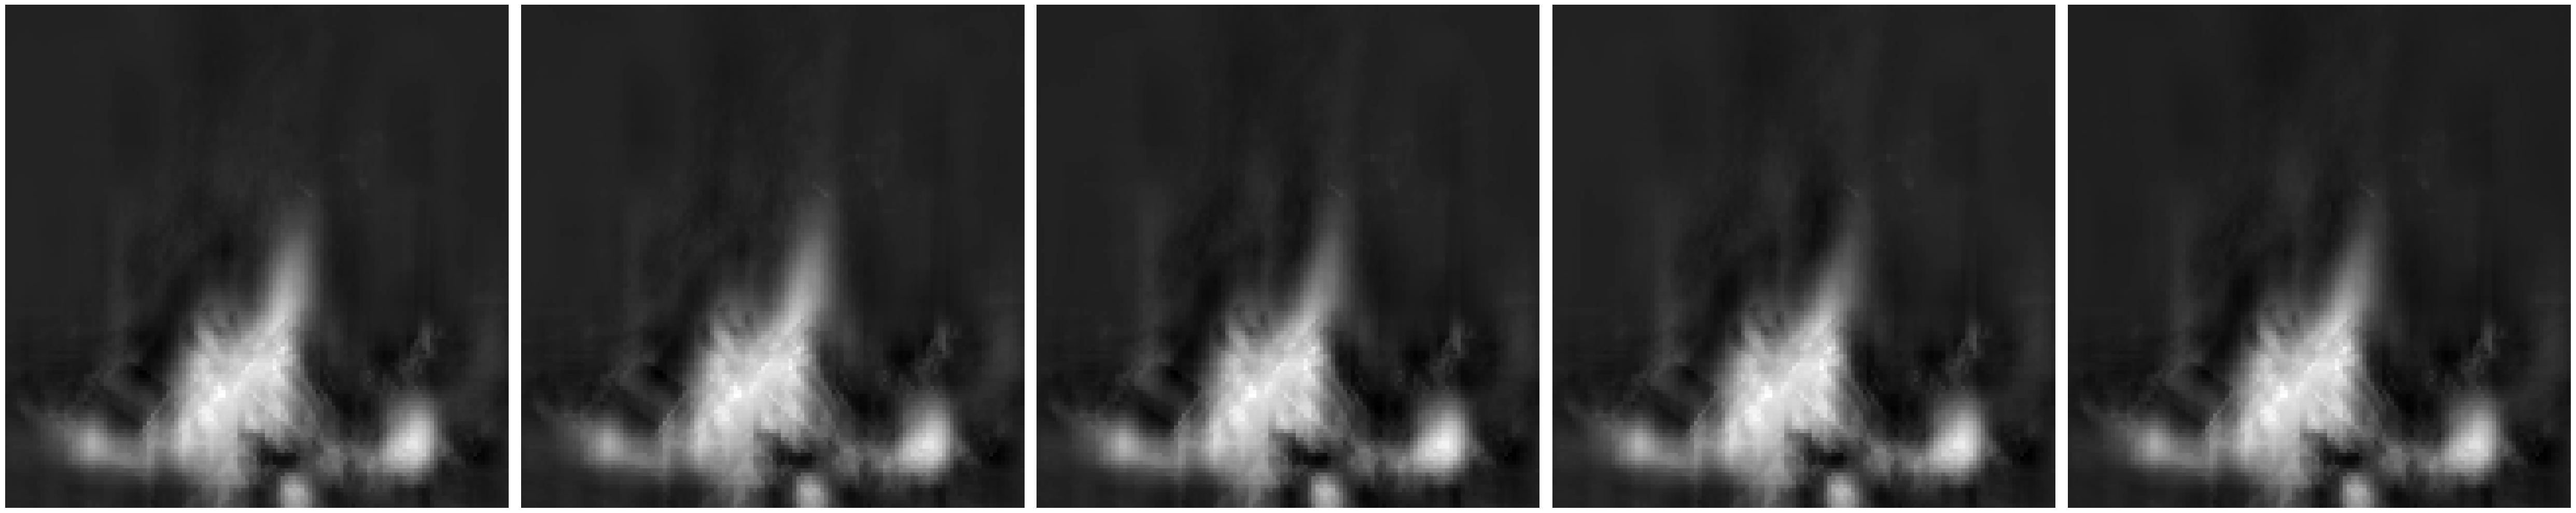
\includegraphics[width=\textwidth]{visuals/Underconstrained_flicker_g1_c4_10.png}
	\end{subfigure}
	\begin{subfigure}{\textwidth}
		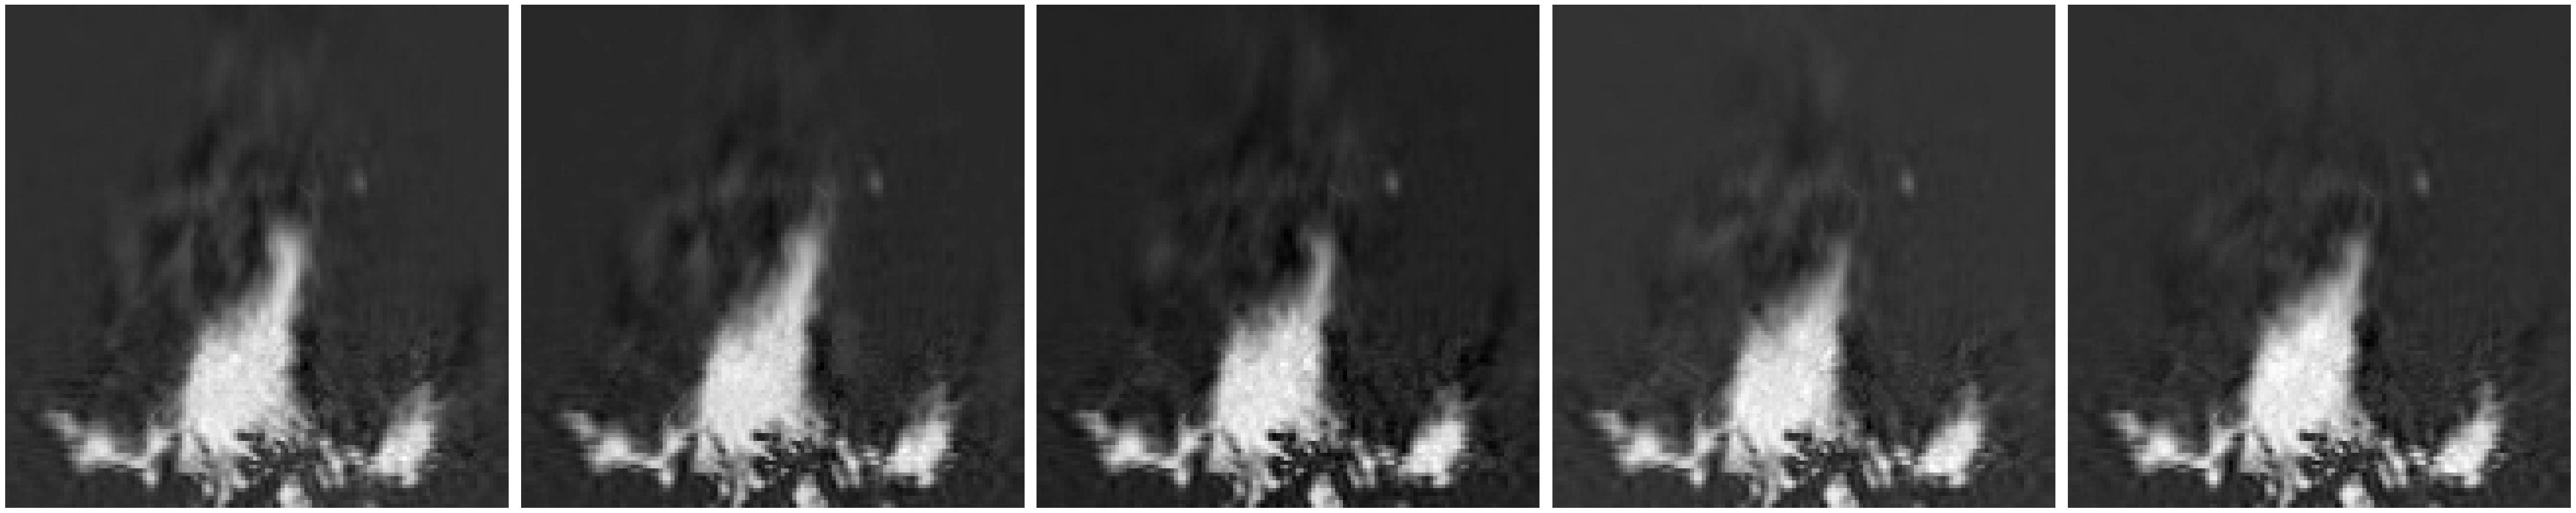
\includegraphics[width=\textwidth]{visuals/Underconstrained_flicker_g1_c4_50.png}
	\end{subfigure}
	\begin{subfigure}{\textwidth}
		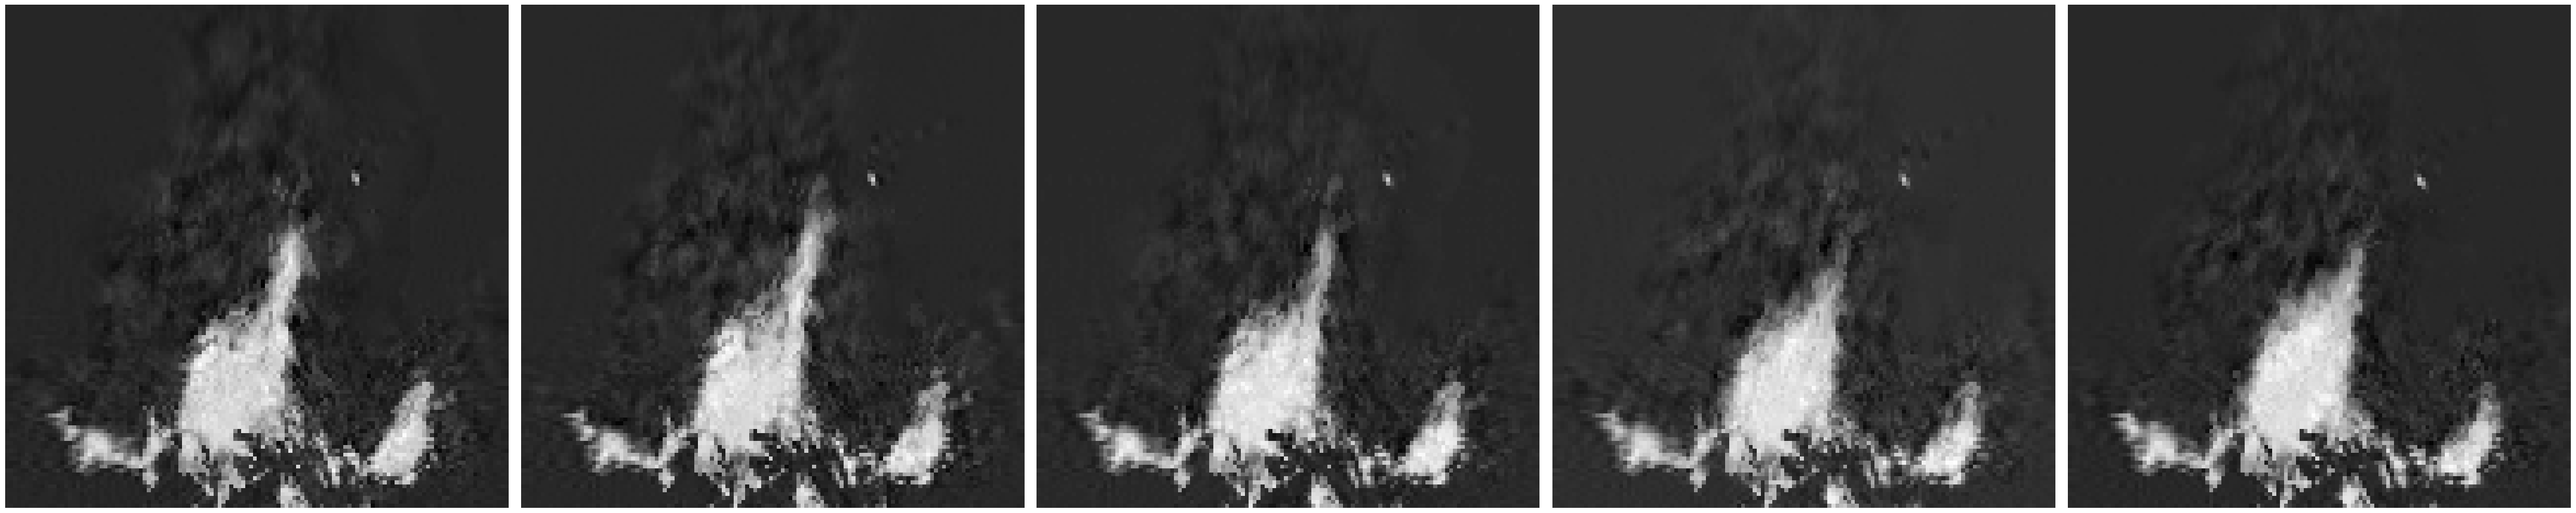
\includegraphics[width=\textwidth]{visuals/Underconstrained_flicker_g1_c4_100.png}
	\end{subfigure}
	\begin{subfigure}{\textwidth}
		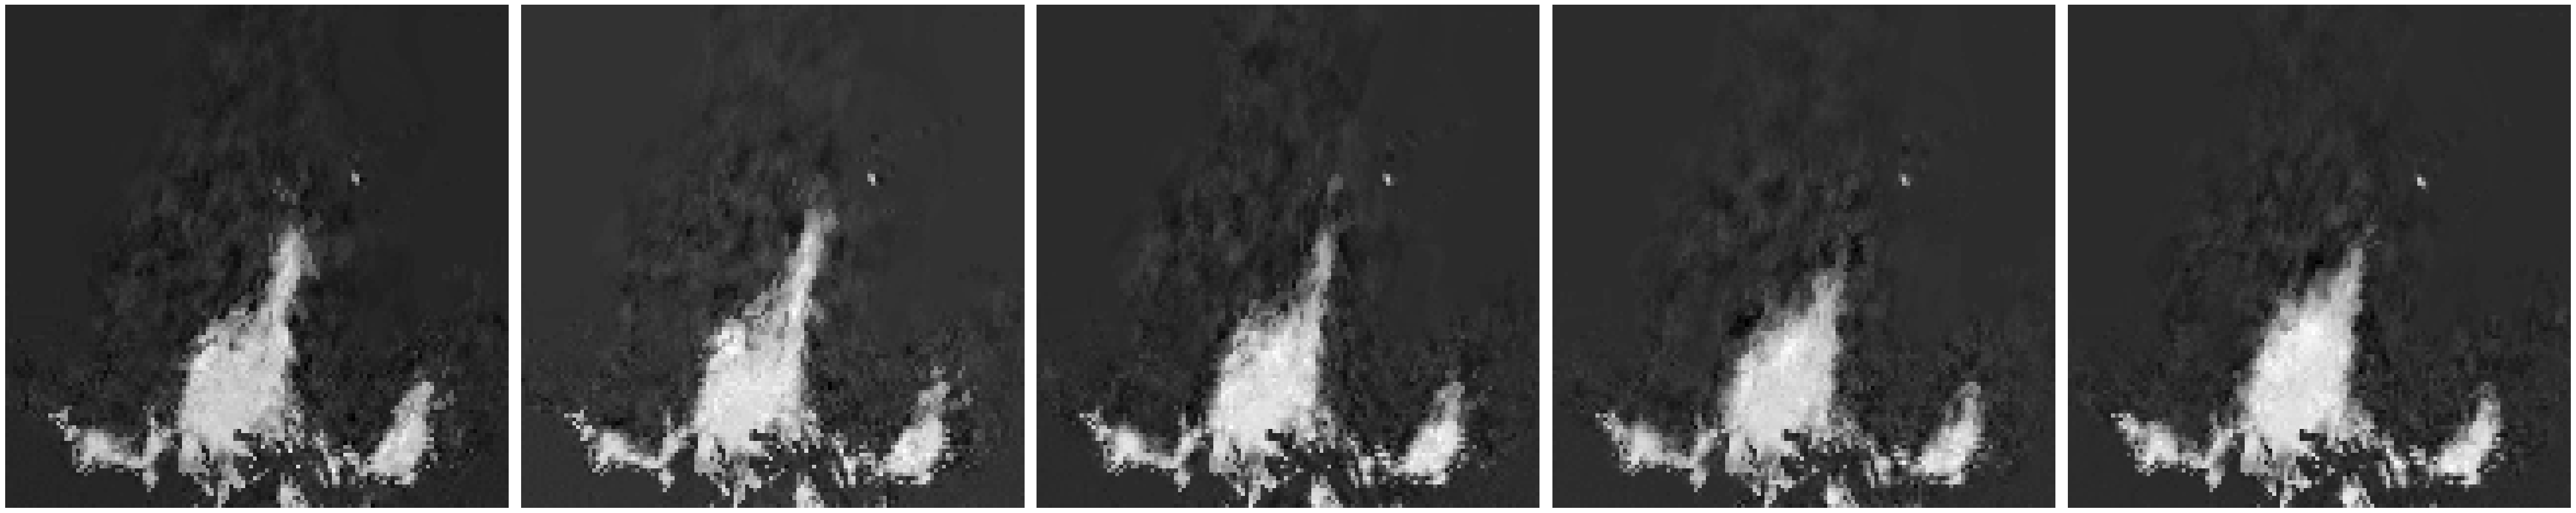
\includegraphics[width=\textwidth]{visuals/Underconstrained_flicker_g1_c4_128.png}
	\end{subfigure}
	\begin{subfigure}{\textwidth}
		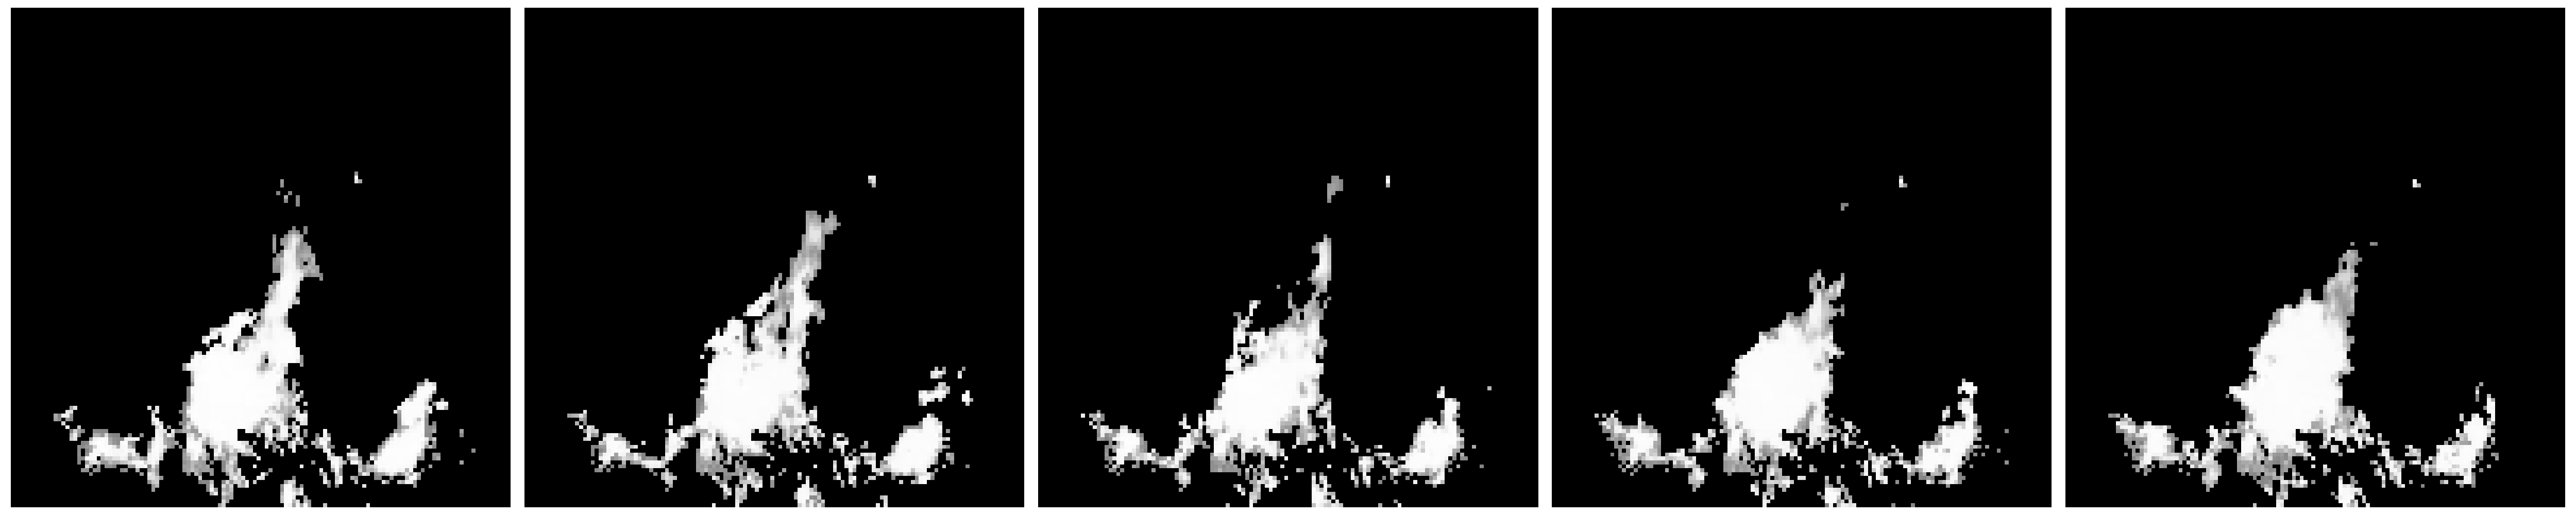
\includegraphics[width=\textwidth]{visuals/Underconstrained_flicker_g1_c4.png}
	\end{subfigure}
	\caption{Reconstruction of a video with 272 frames, original on the bottom}
	\label{fig:reconstruction-1}
\end{figure}

\begin{figure}
	\centering
	\begin{subfigure}{\textwidth}
		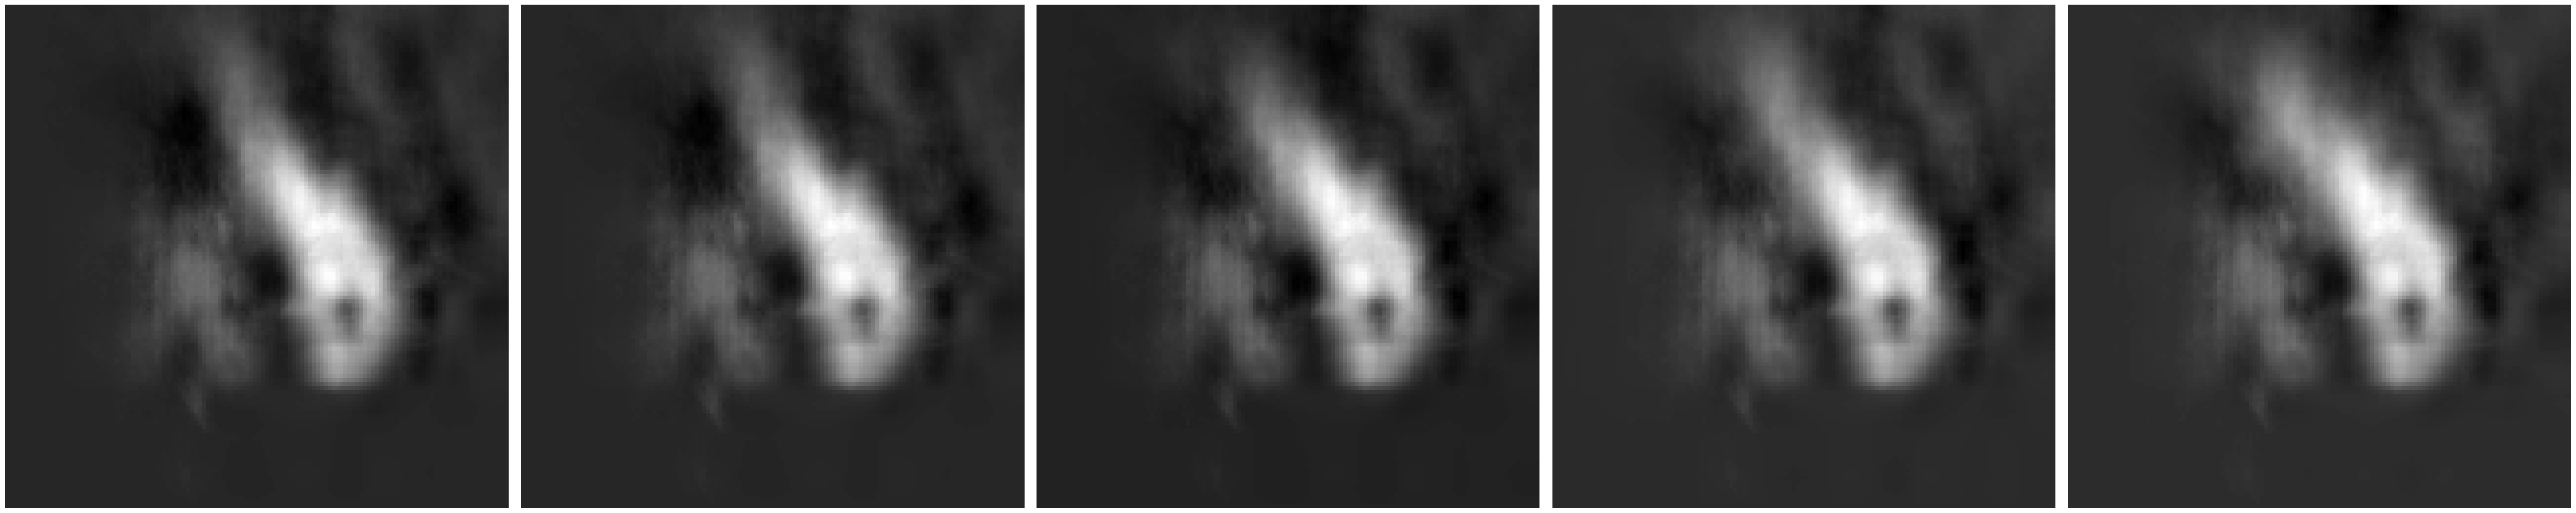
\includegraphics[width=\textwidth]{visuals/Underconstrained_flicker_g1_c28_10.png}
	\end{subfigure}
	\begin{subfigure}{\textwidth}
		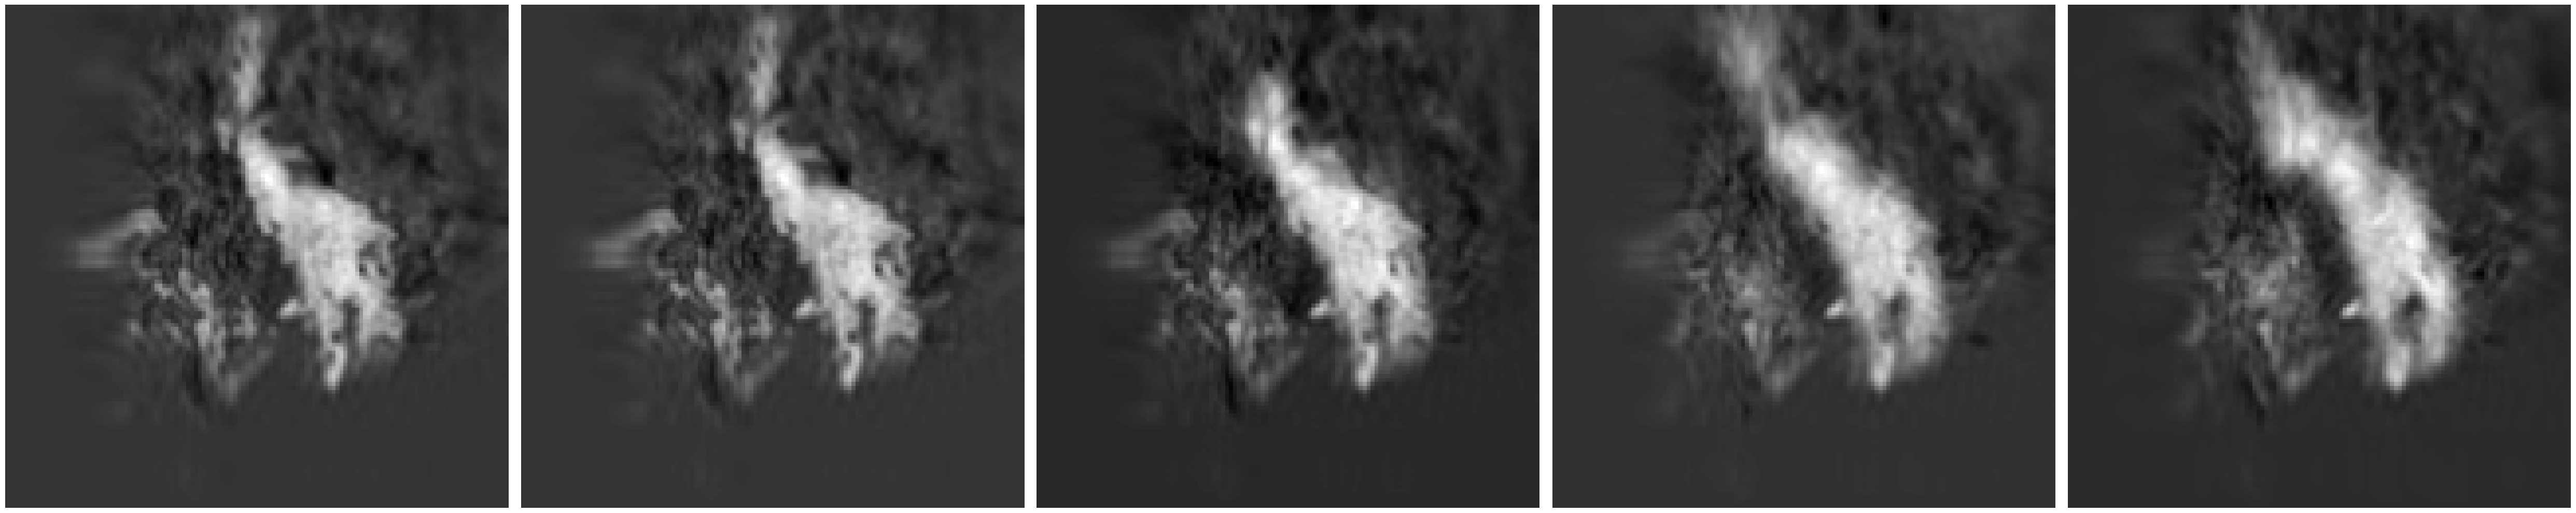
\includegraphics[width=\textwidth]{visuals/Underconstrained_flicker_g1_c28_50.png}
	\end{subfigure}
	\begin{subfigure}{\textwidth}
		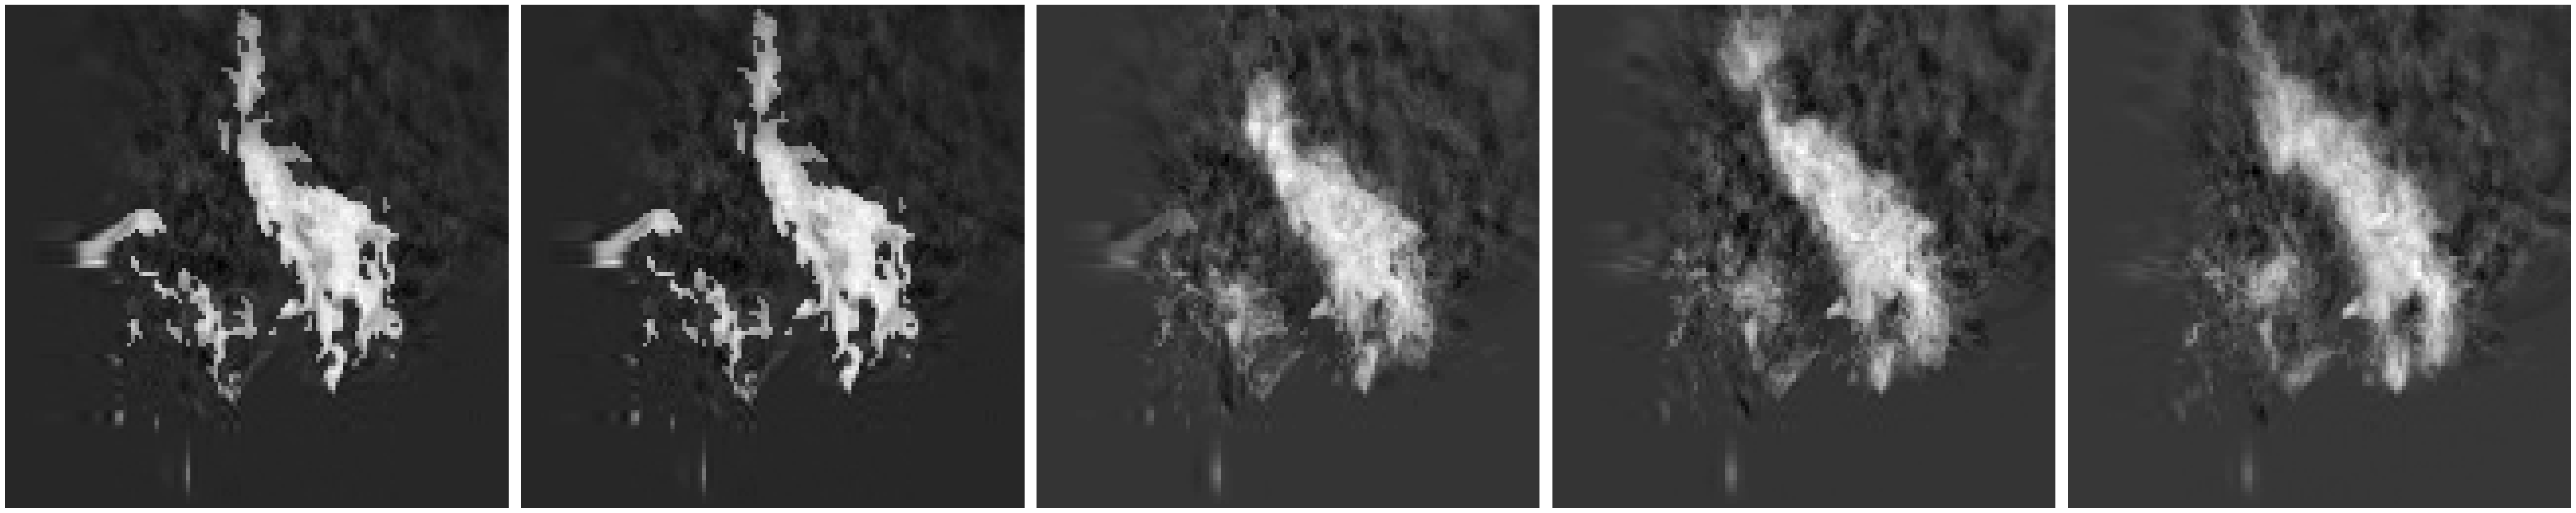
\includegraphics[width=\textwidth]{visuals/Underconstrained_flicker_g1_c28_100.png}
	\end{subfigure}
	\begin{subfigure}{\textwidth}
		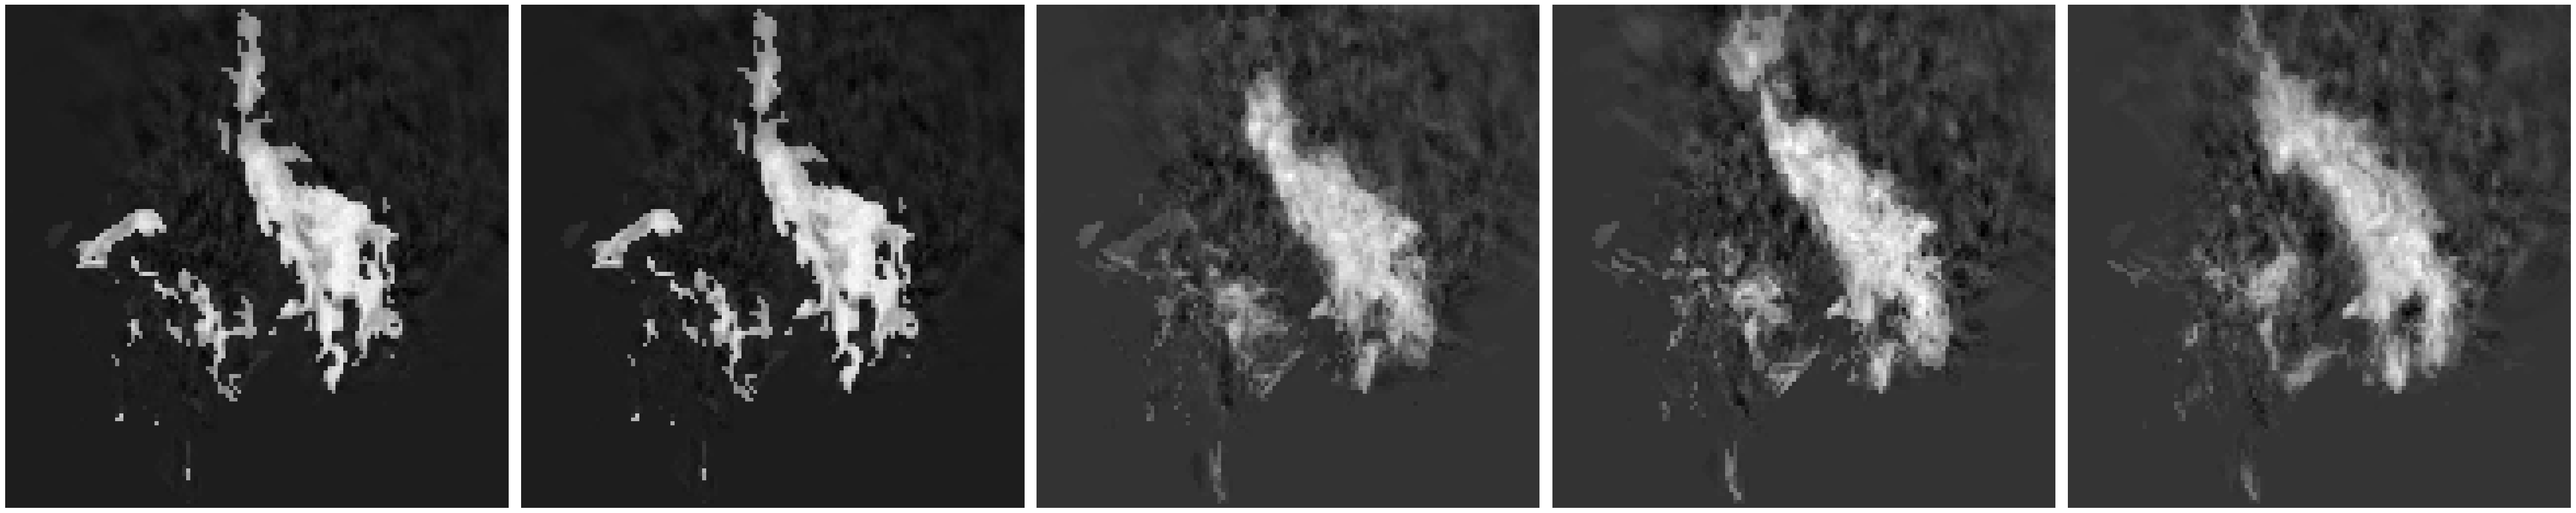
\includegraphics[width=\textwidth]{visuals/Underconstrained_flicker_g1_c28_128.png}
	\end{subfigure}
	\begin{subfigure}{\textwidth}
		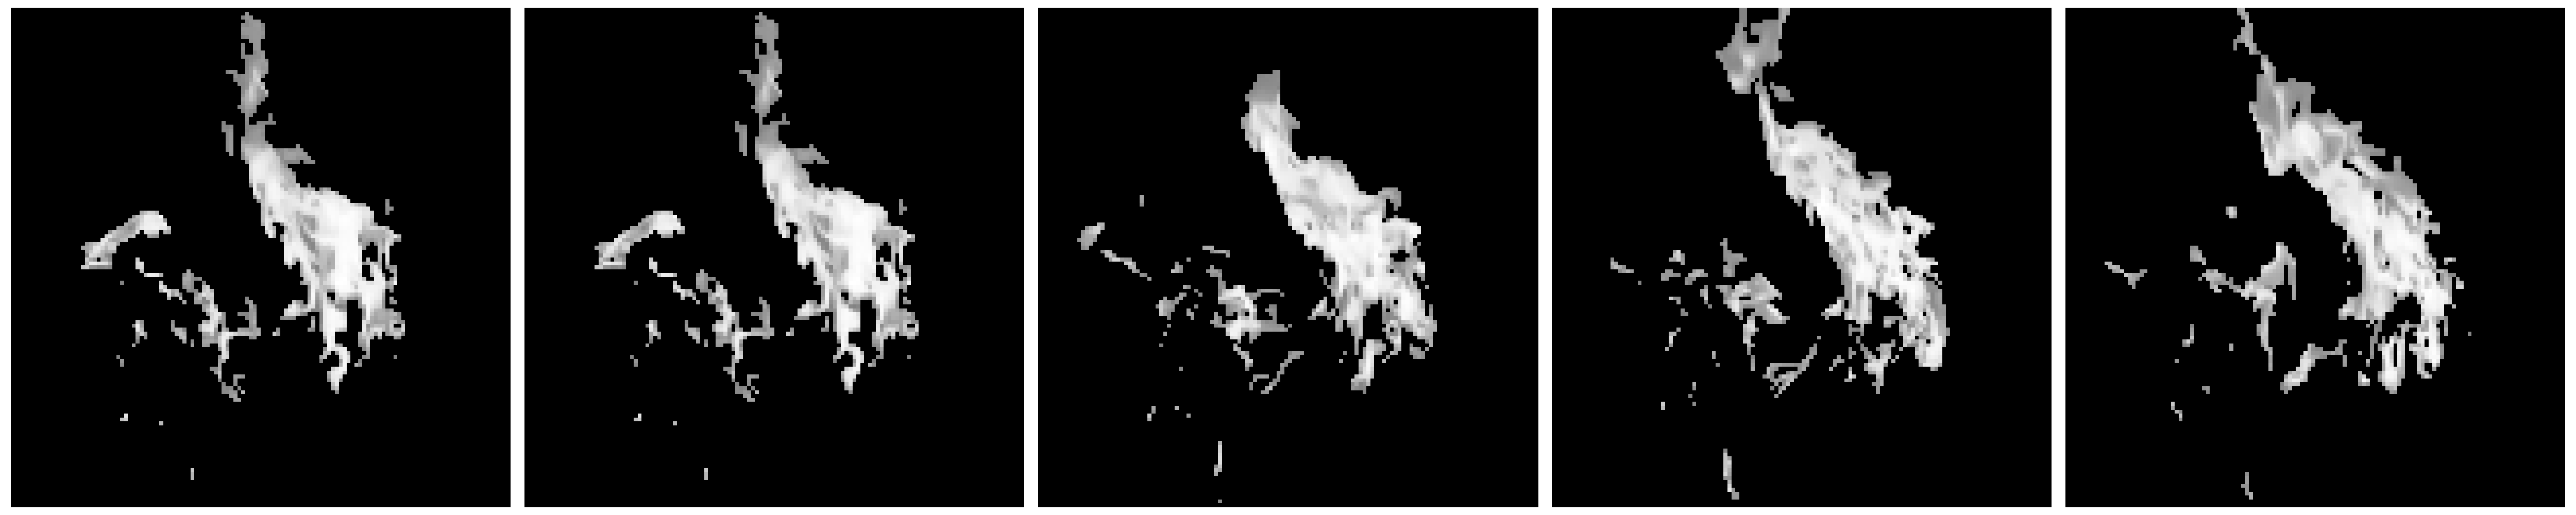
\includegraphics[width=\textwidth]{visuals/Underconstrained_flicker_g1_c28.png}
	\end{subfigure}
	\caption{Reconstruction of a video with 284 frames, original on the bottom}
	\label{fig:reconstruction-2}
\end{figure}

\begin{figure}
	\centering
	\begin{subfigure}{\textwidth}
		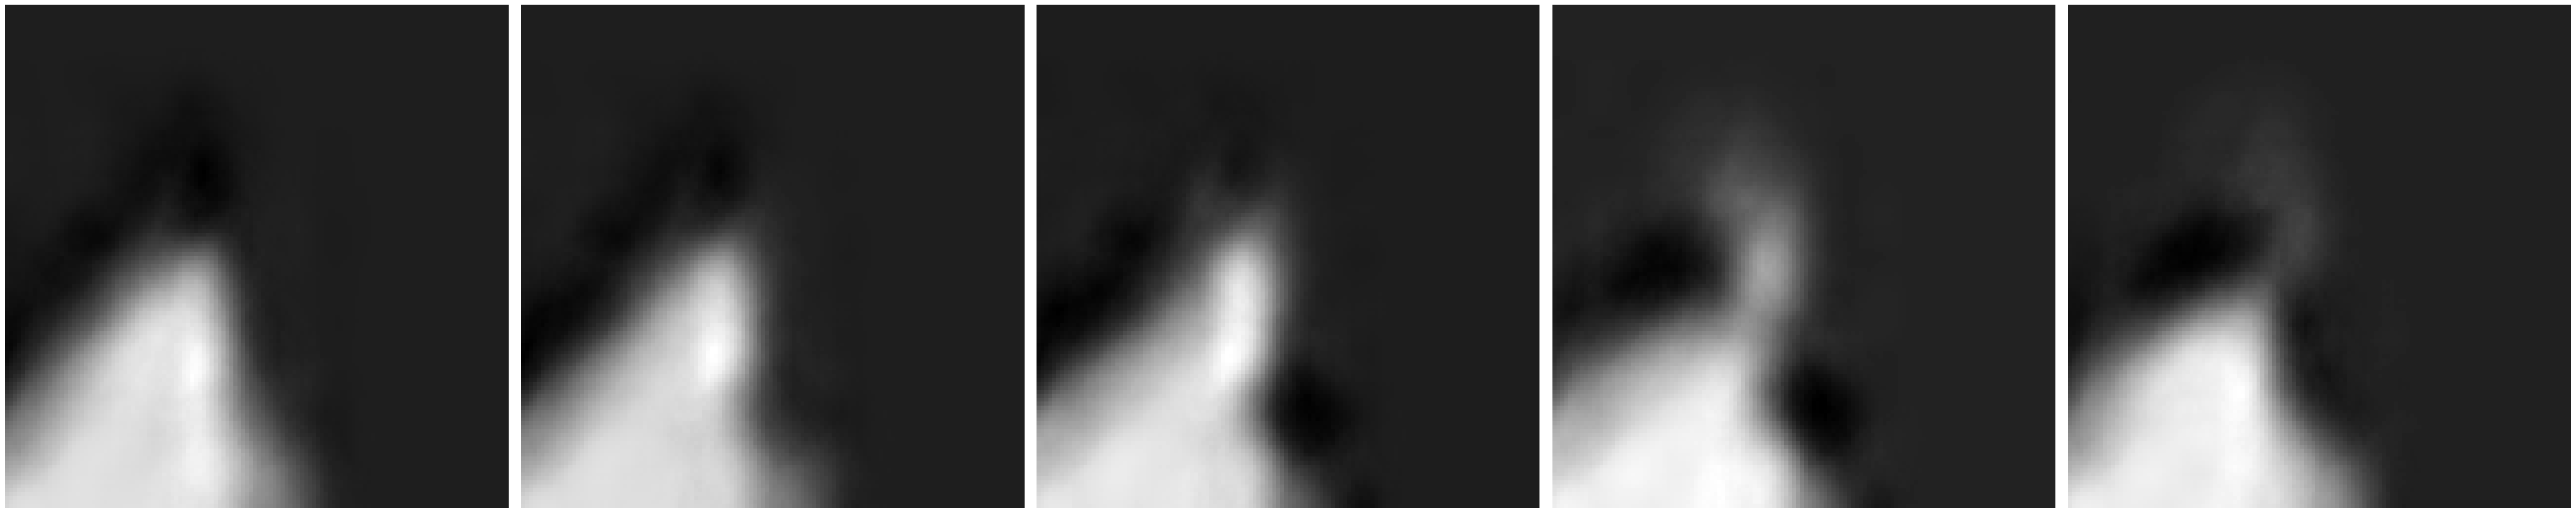
\includegraphics[width=\textwidth]{visuals/Underconstrained_flicker_g1_c111_10.png}
	\end{subfigure}
	\begin{subfigure}{\textwidth}
		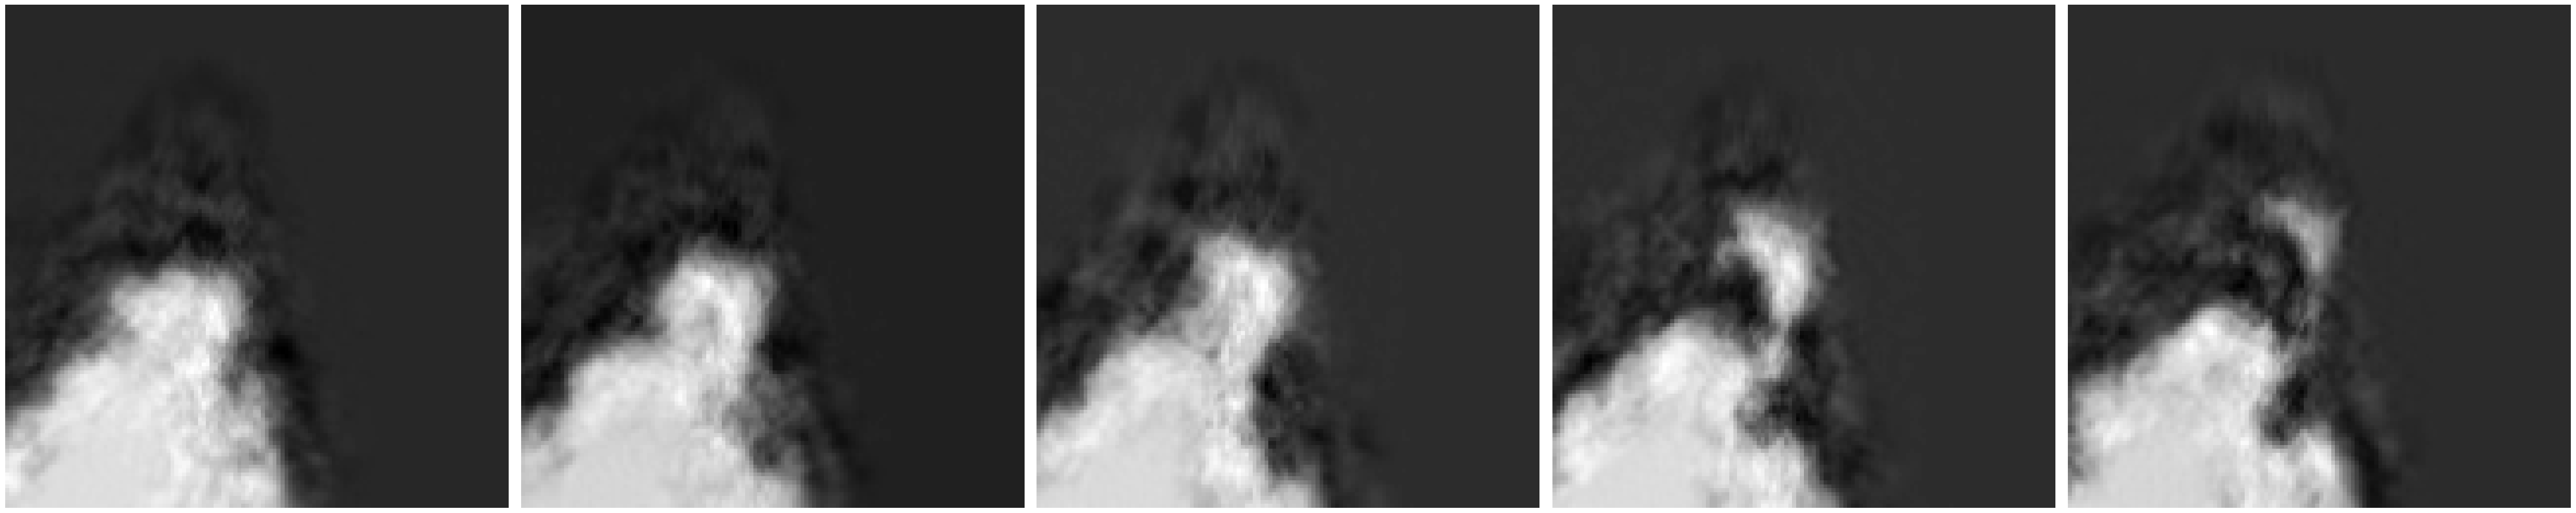
\includegraphics[width=\textwidth]{visuals/Underconstrained_flicker_g1_c111_50.png}
	\end{subfigure}
	\begin{subfigure}{\textwidth}
		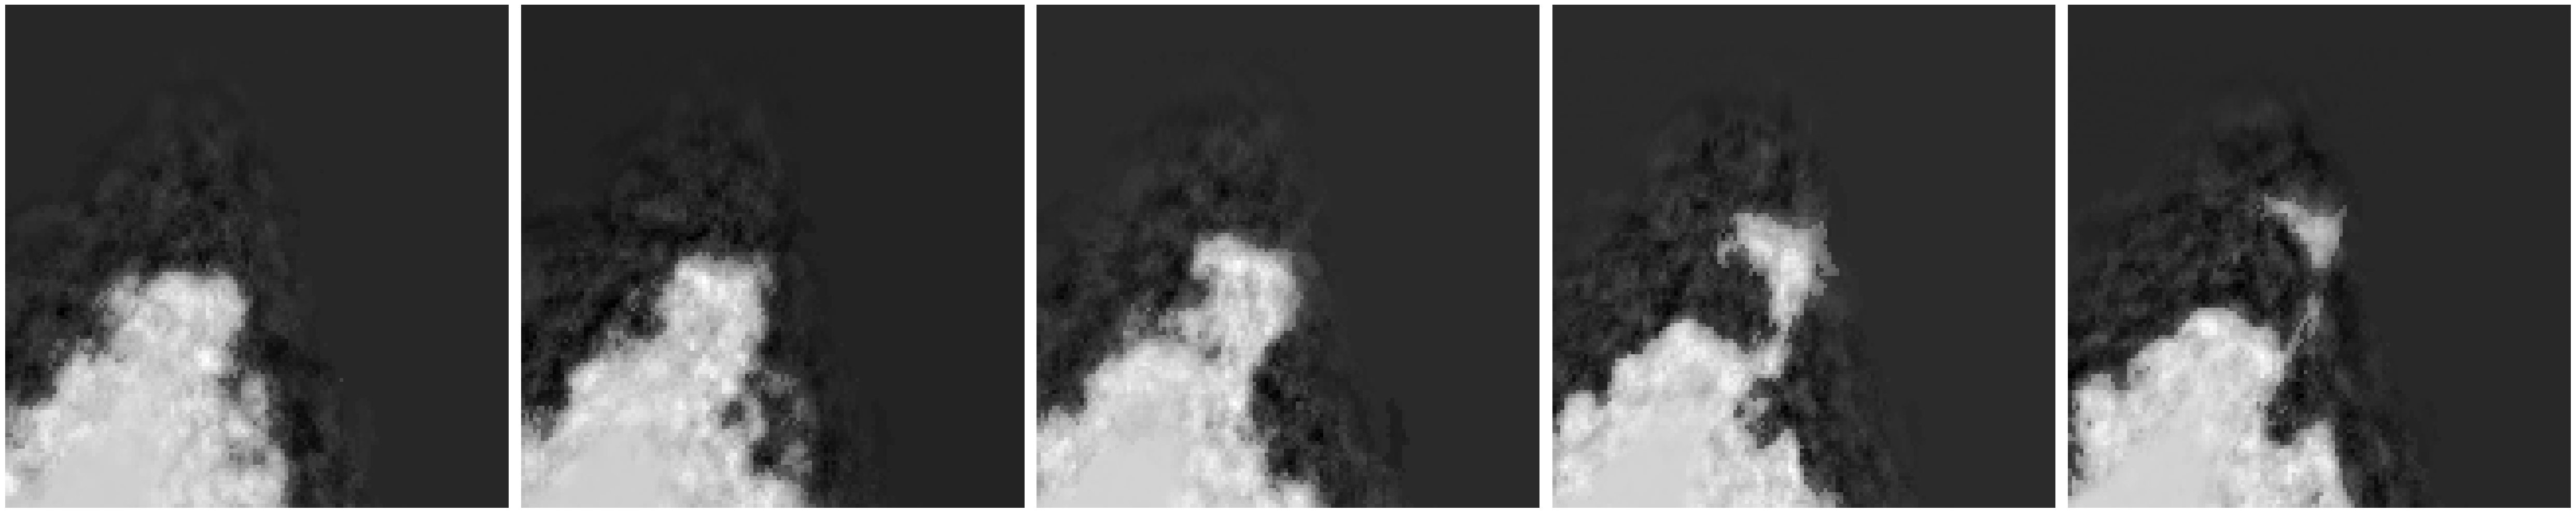
\includegraphics[width=\textwidth]{visuals/Underconstrained_flicker_g1_c111_100.png}
	\end{subfigure}
	\begin{subfigure}{\textwidth}
		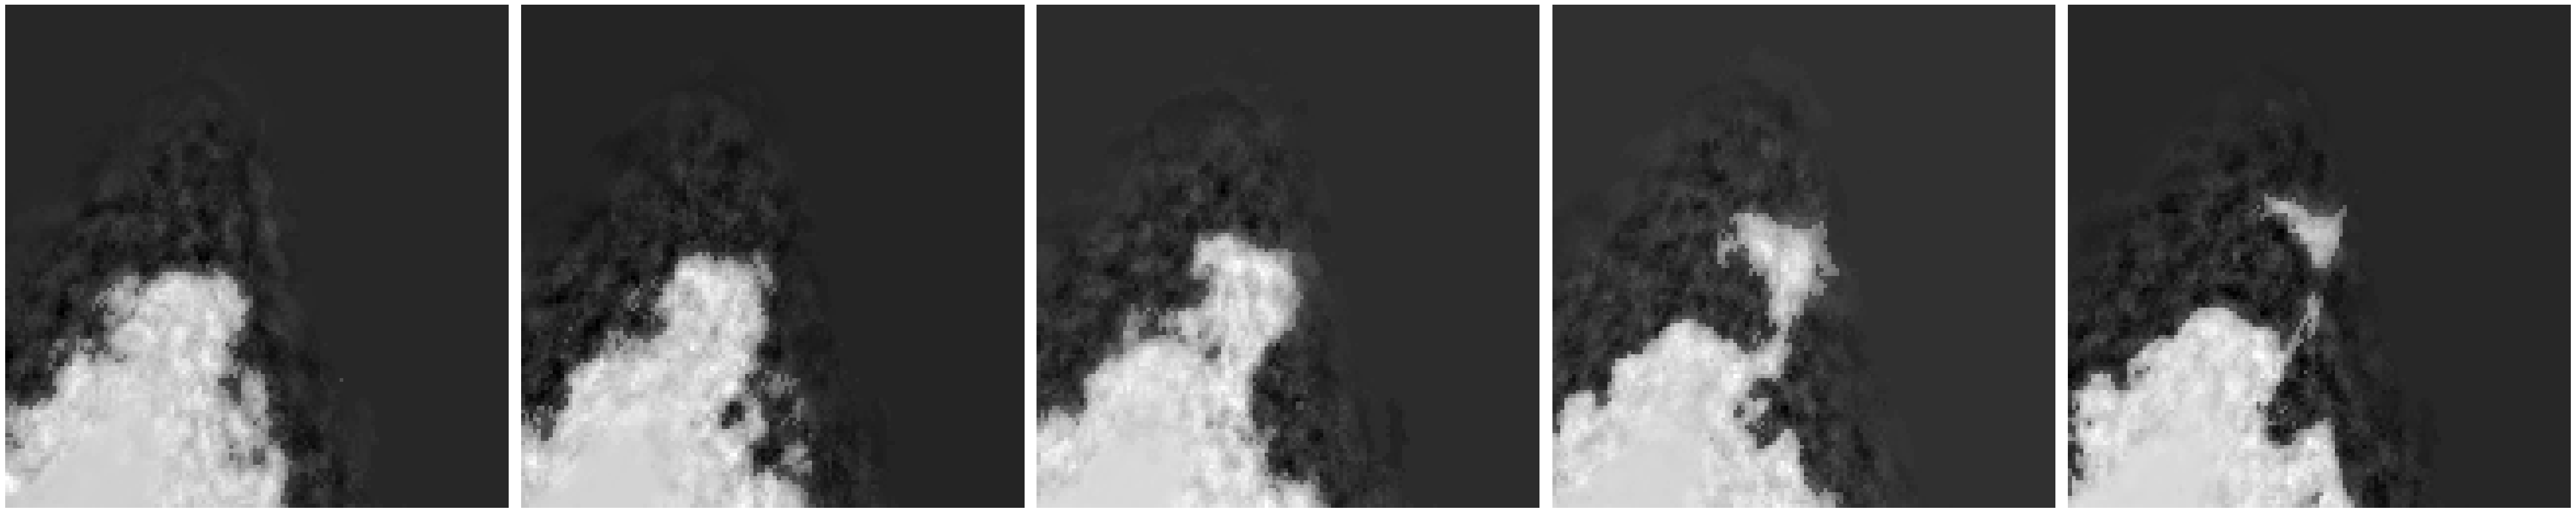
\includegraphics[width=\textwidth]{visuals/Underconstrained_flicker_g1_c111_128.png}
	\end{subfigure}
	\begin{subfigure}{\textwidth}
		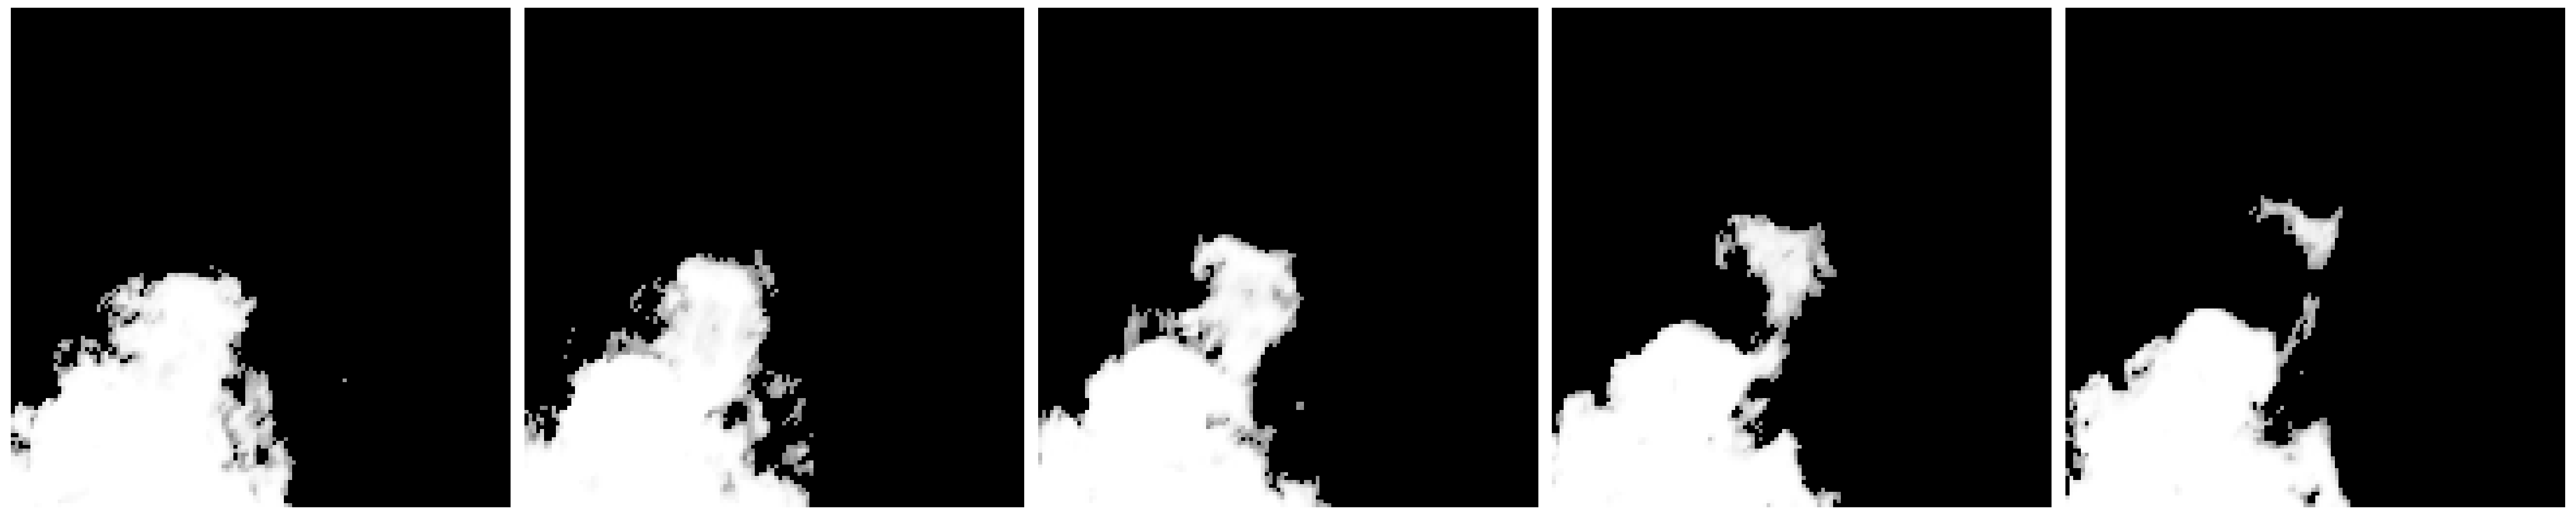
\includegraphics[width=\textwidth]{visuals/Underconstrained_flicker_g1_c111.png}
	\end{subfigure}
	\caption{Reconstruction of a video with 299 frames, original on the bottom}
	\label{fig:reconstruction-3}
\end{figure}

\subsection{Synthesis}
Similarly, we try "training" a model on the tensors for each of the shown flame videos, and then synthesise new frames by running the model forward in time, sampling $\bf v(t)$s from the standard multivariate gaussian.\bigskip

For synthesis, I've used a rank of 100 for all modes, and the results are shown in Figures \ref{fig:synthesis-1}, \ref{fig:synthesis-2}, and \ref{fig:synthesis-3}. As we can see, the synthesised frames are distinct enough from the original frames to be considered new frames, due to the randomly sampled noise, but they still retain the general dynamics of the flames in the original flames. \bigskip

In Table \ref{tab:synthesis}, I've also indicated the mean residuals and the time taken for synthesising 100 frames. The mean residuals are quite low, indicating that the linear model is quite good at capturing the dynamics of the flames. Furthermore, the technique is also quite efficient, able to synthesise 100 frames in under 5 seconds, which means it is quite feasible to use this technique for real-time applications.\bigskip

\begin{table}
	\centering
	\begin{tabular}{|c|c|c|c|}
		\hline \textbf{Scene} & \textbf{Mean Residual} & \textbf{Max Residual} & \textbf{Time (s)}\\
		\hline 1 & 1.058e-5 & 0.0025 & 3.7\\
		\hline 2 & 1.690e-5 & 0.0038 & 4.1\\
		\hline 3 & 1.387e-5 & 0.0026 & 3.9\\
		\hline
	\end{tabular}
	\caption{HOSVD synthesis time \& mean residuals for different approximations}
	\label{tab:synthesis}
\end{table}

\begin{figure}
	\centering
	\begin{subfigure}{\textwidth}
		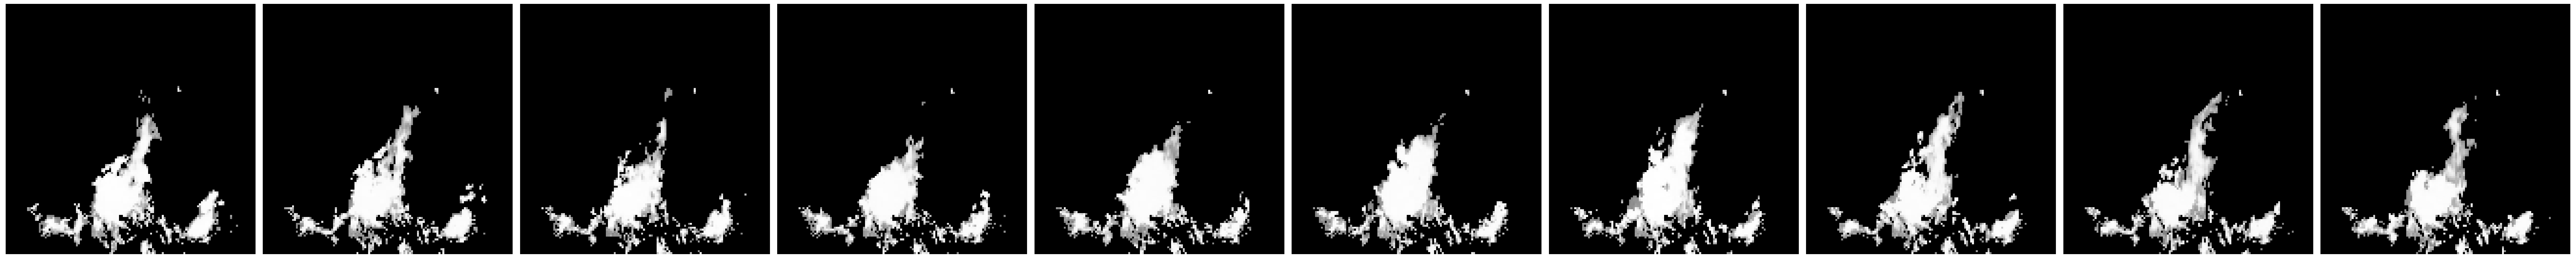
\includegraphics[width=\textwidth]{visuals/Underconstrained_flicker_g1_c4_f10.png}
	\end{subfigure}
	\begin{subfigure}{\textwidth}
		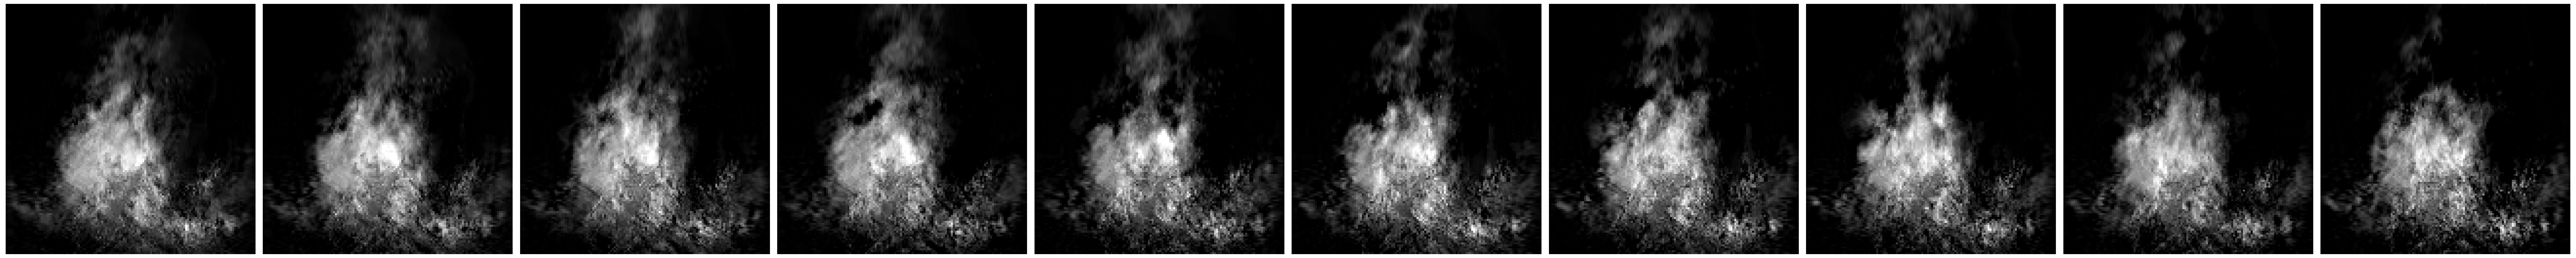
\includegraphics[width=\textwidth]{visuals/Underconstrained_flicker_g1_c4_s0_synth.png}
	\end{subfigure}
	\begin{subfigure}{\textwidth}
		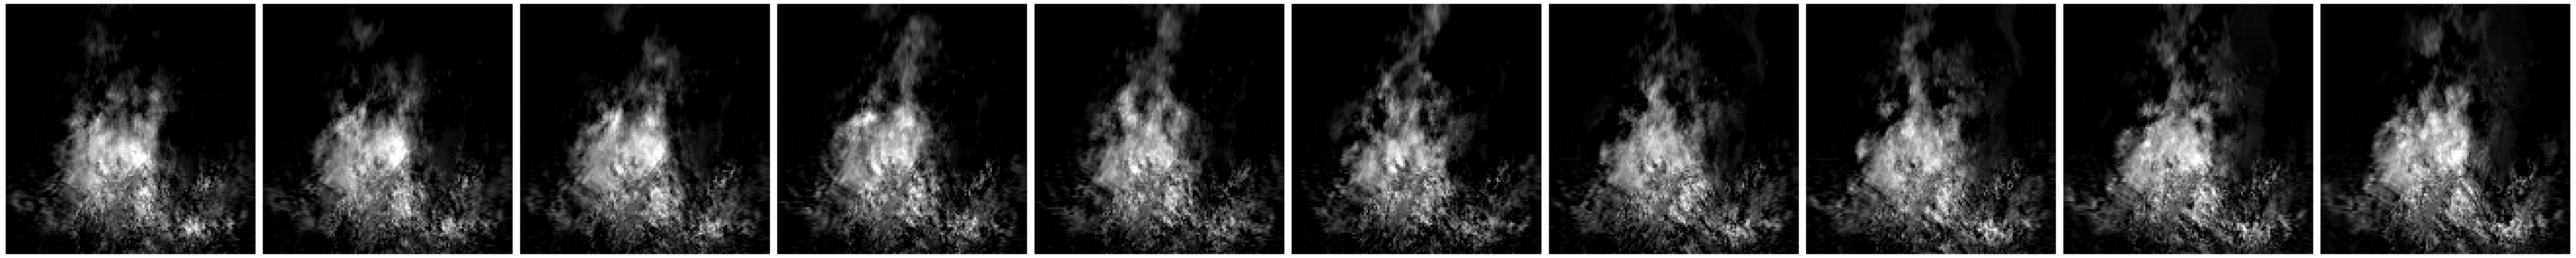
\includegraphics[width=\textwidth]{visuals/Underconstrained_flicker_g1_c4_s10_synth.png}
	\end{subfigure}
	\begin{subfigure}{\textwidth}
		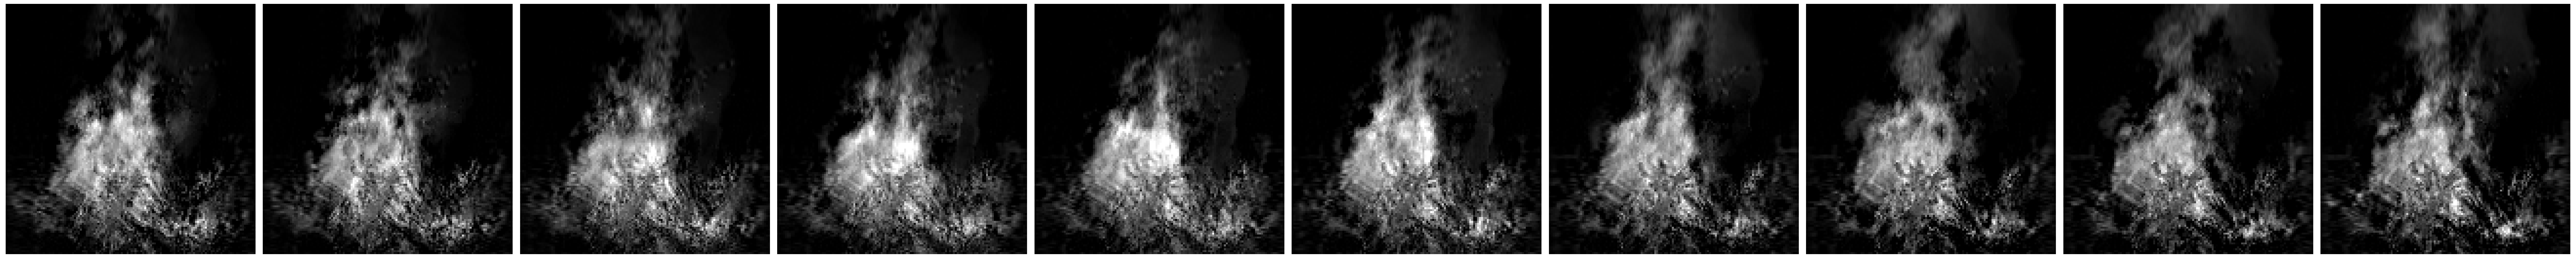
\includegraphics[width=\textwidth]{visuals/Underconstrained_flicker_g1_c4_s20_synth.png}
	\end{subfigure}
	\caption{Synthesis results for scene 1, first row is original, rest are thirty frames from the synthesised video}
	\label{fig:synthesis-1}
\end{figure}

\begin{figure}
	\centering
	\begin{subfigure}{\textwidth}
		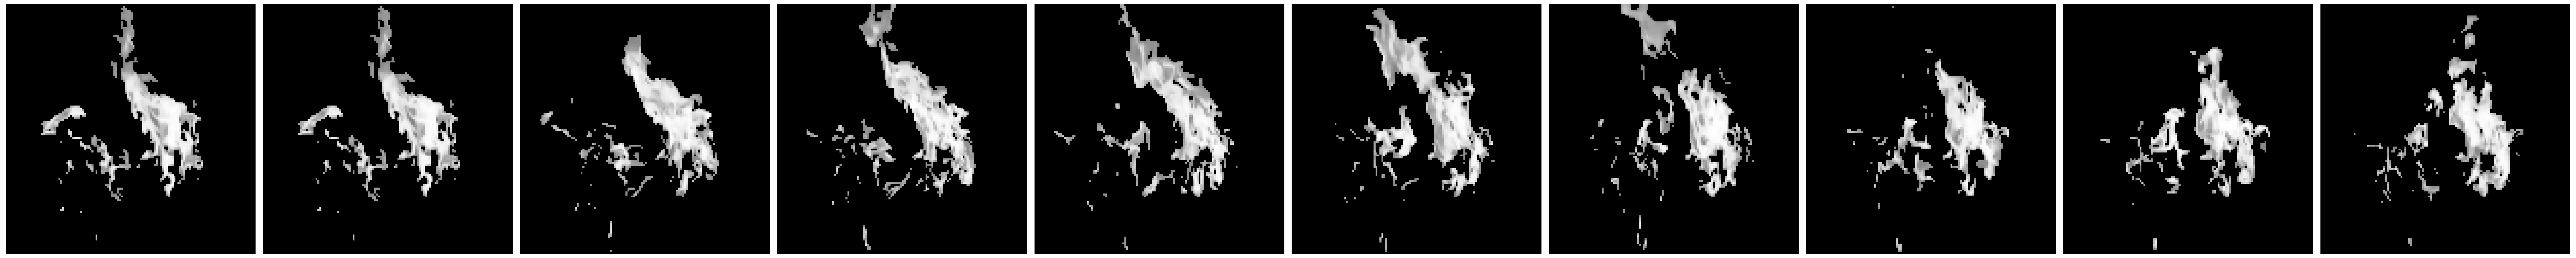
\includegraphics[width=\textwidth]{visuals/Underconstrained_flicker_g1_c28_f10.png}
	\end{subfigure}
	\begin{subfigure}{\textwidth}
		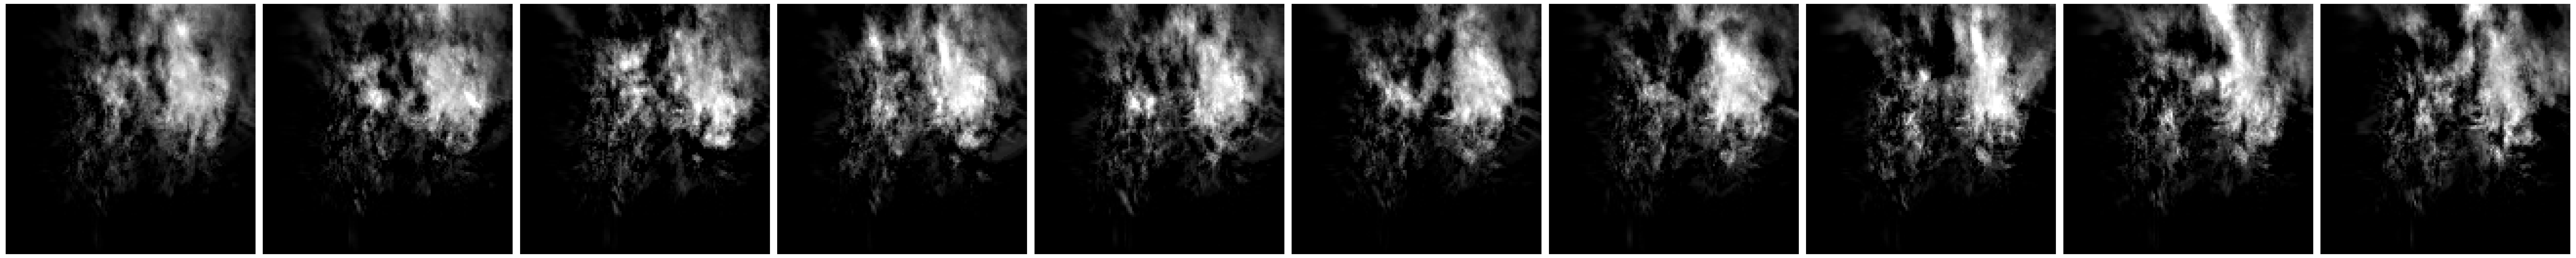
\includegraphics[width=\textwidth]{visuals/Underconstrained_flicker_g1_c28_s0_synth.png}
	\end{subfigure}
	\begin{subfigure}{\textwidth}
		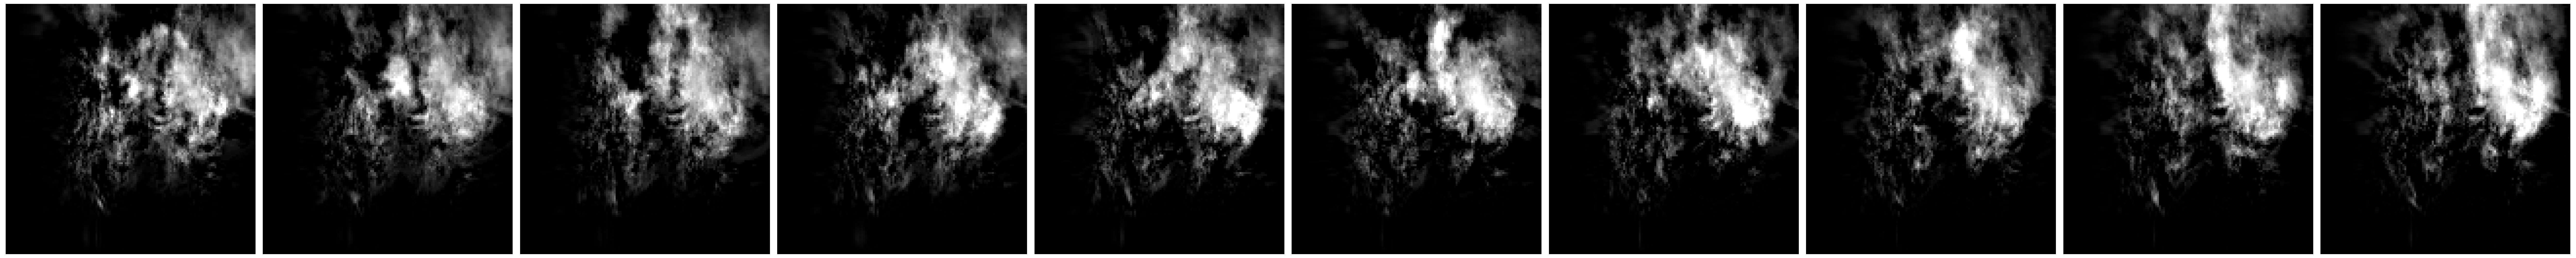
\includegraphics[width=\textwidth]{visuals/Underconstrained_flicker_g1_c28_s10_synth.png}
	\end{subfigure}
	\begin{subfigure}{\textwidth}
		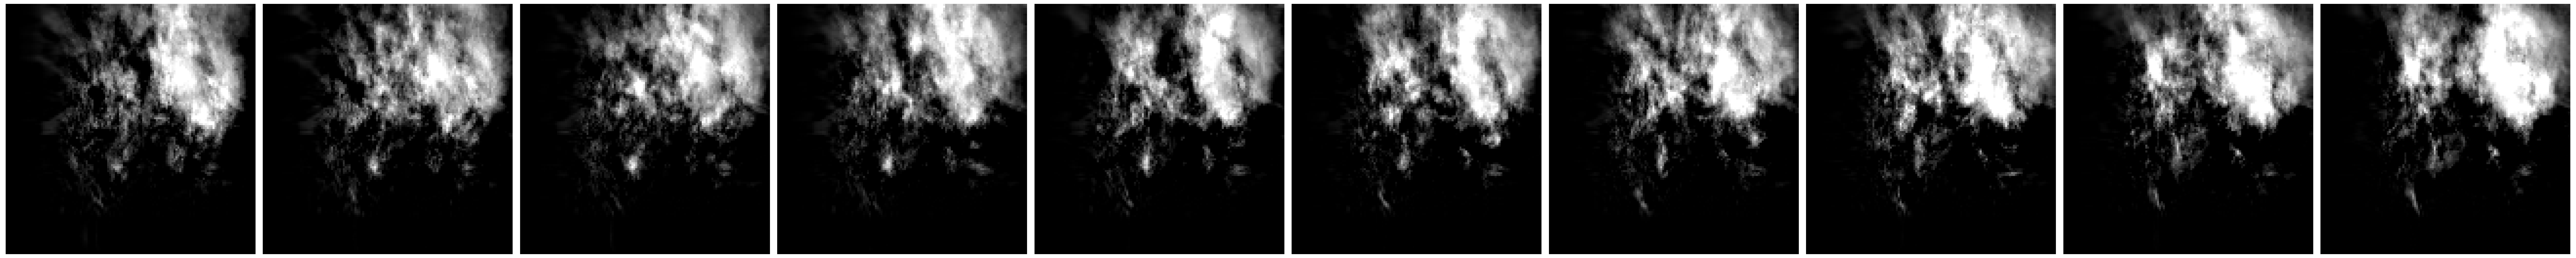
\includegraphics[width=\textwidth]{visuals/Underconstrained_flicker_g1_c28_s20_synth.png}
	\end{subfigure}
	\caption{Synthesis results for scene 2, first row is original, rest are thirty frames from the synthesised video}
	\label{fig:synthesis-2}
\end{figure}

\begin{figure}
	\centering
	\begin{subfigure}{\textwidth}
		\includegraphics[width=\textwidth]{visuals/Underconstrained_flicker_g1_c111_f10.png}
	\end{subfigure}
	\begin{subfigure}{\textwidth}
		\includegraphics[width=\textwidth]{visuals/Underconstrained_flicker_g1_c111_s0_synth.png}
	\end{subfigure}
	\begin{subfigure}{\textwidth}
		\includegraphics[width=\textwidth]{visuals/Underconstrained_flicker_g1_c111_s10_synth.png}
	\end{subfigure}
	\begin{subfigure}{\textwidth}
		\includegraphics[width=\textwidth]{visuals/Underconstrained_flicker_g1_c111_s20_synth.png}
	\end{subfigure}
	\caption{Synthesis results for scene 3, first row is original, rest are thirty frames from the synthesised video}
	\label{fig:synthesis-3}
\end{figure}

What seems to be clear is that the system has a harder time modelling the more restrained "masked out" flames (firewood etc. removed by threshold) in scenes 1 \& 2 than the more unrestrained blobby frame in scene 3. This is possibly because the masked regions in the first two scenes add spatial complexity, which would require higher spatial ranks to model effectively. Further postprocessing (or data preprocessing) may be able to get more realistic or visually appealing results, but I am quite happy with the results as they are, since we have at least effectively been able to synthesise a new flame sequence from a low-rank approximation of the original.

\newpage
\bibliographystyle{plain}
\bibliography{refs}

\end{document}